\subsection{骑手端功能实现}

骑手端主要面向配送人员，提供订单查看、订单搜索、进入订单通信和异常申请等功能。骑手端的实现重点是满足配送沟通需求，同时严格限制敏感信息展示范围。与传统外卖系统中骑手可能看到用户真实姓名、联系方式或详细备注不同，FoodShield 骑手端只展示完成配送所需的订单信息和通信入口，不展示用户真实身份，不展示用户 PID，也不展示用户备注和标签原文。

骑手进入系统后，可以查看当前可处理订单，也可以根据订单号搜索目标订单。骑手端在进入通信页面前，需要通过订单状态校验。服务器只有在订单处于可通信状态时，才允许骑手加入对应订单房间。该机制可以防止任意骑手随意进入其他订单的通信通道。

\begin{figure}[H]
    \centering
    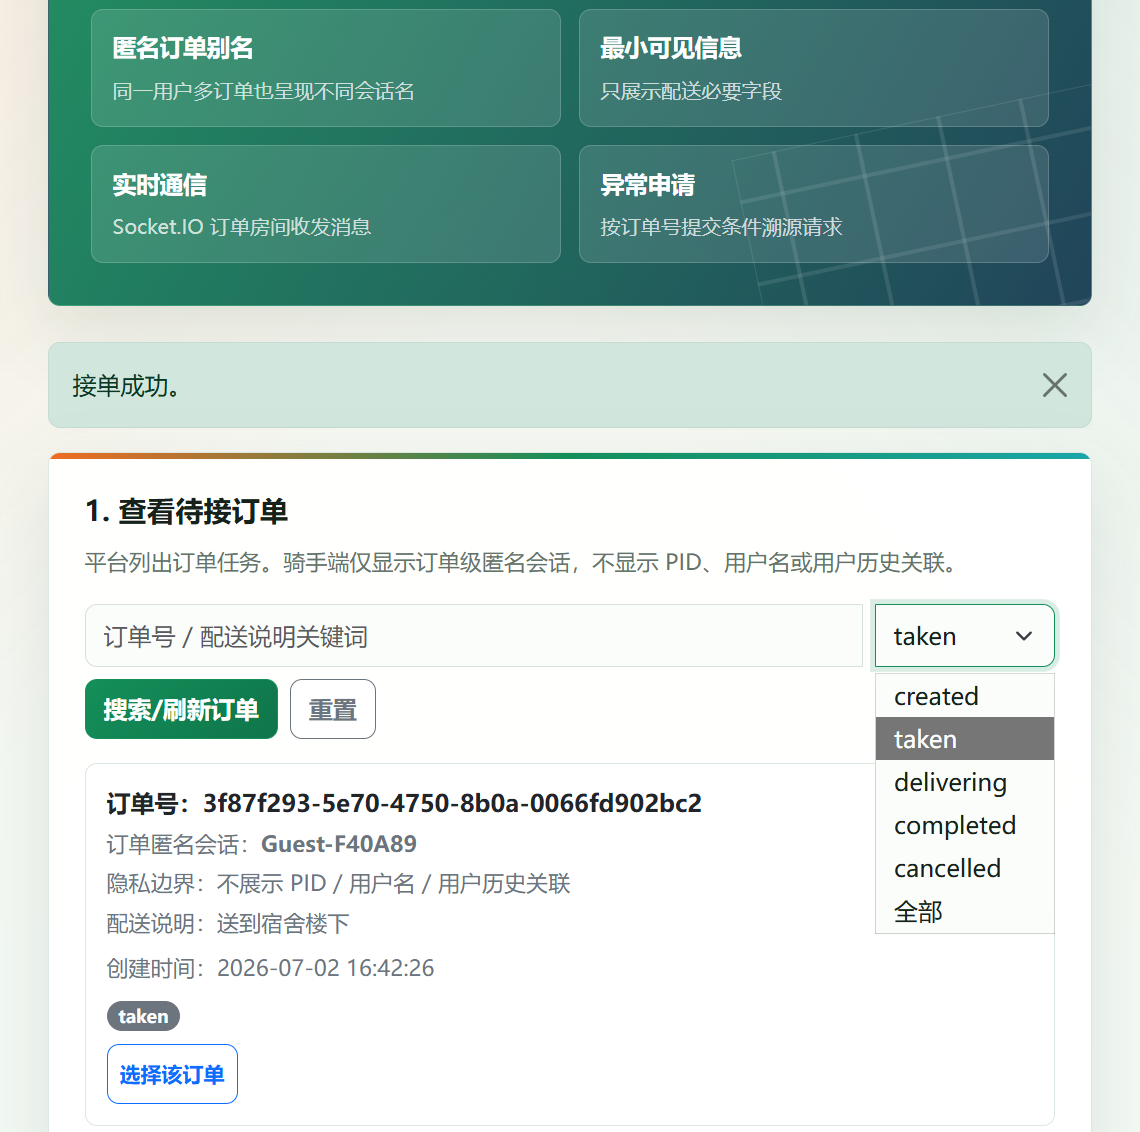
\includegraphics[width=0.9\textwidth]{content/chapter4/rider_orders.png}
    \caption{骑手端订单管理界面}
    \label{fig:rider-orders}
\end{figure}

骑手加入订单通信房间后，可以与用户进行实时通信。前端页面仅展示发送方角色、消息内容和时间等必要信息，不展示用户 PID 或真实用户名。即使后端消息记录中包含发送方匿名标识，骑手端页面也不会将该字段渲染出来，从而降低骑手通过固定标识进行跨订单关联的风险。

\begin{figure}[H]
    \centering
    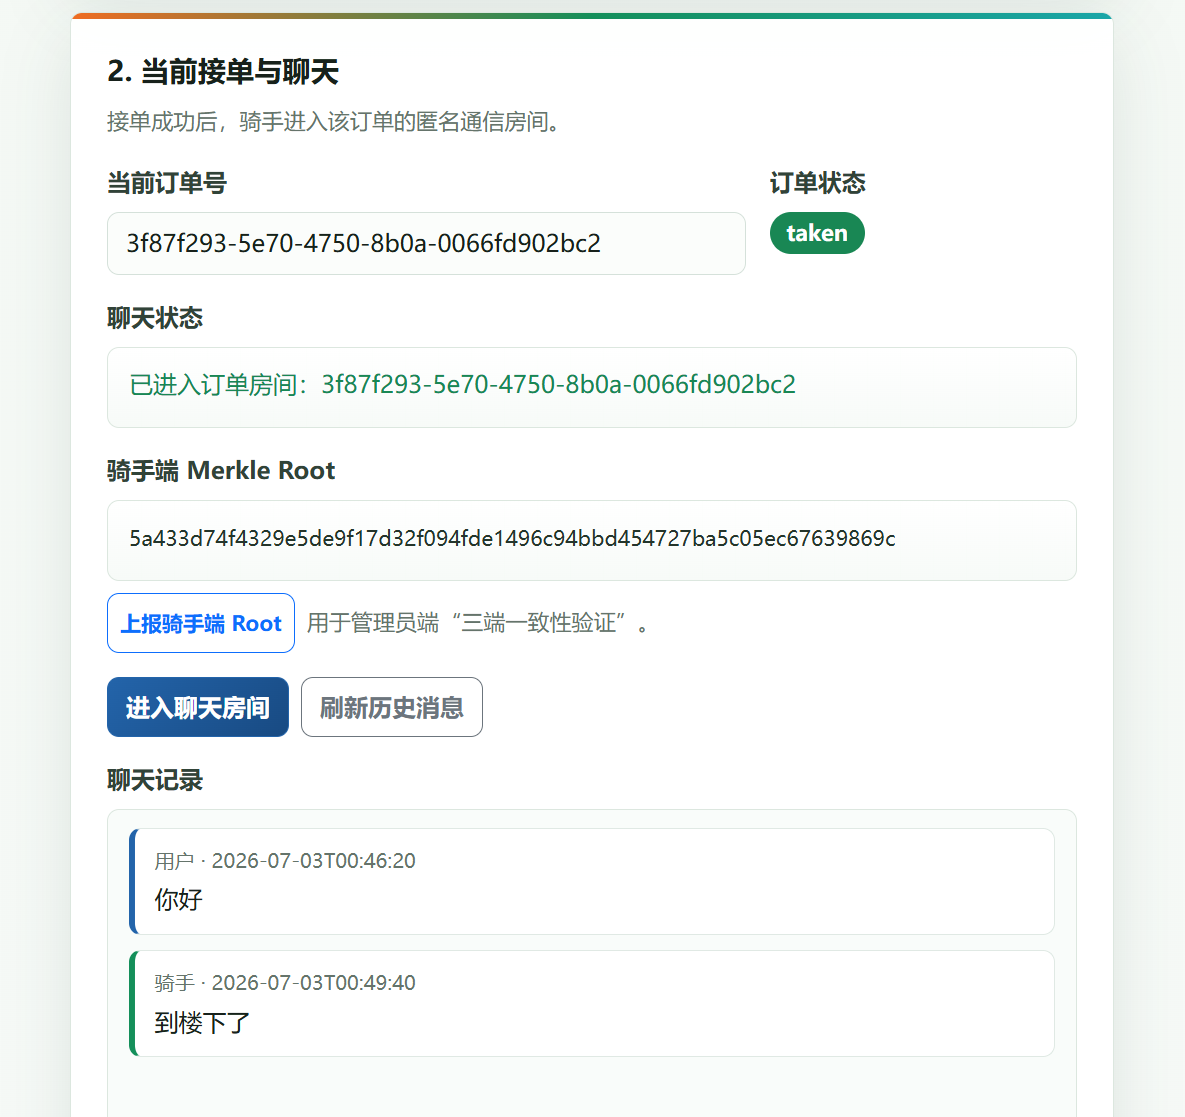
\includegraphics[width=0.9\textwidth]{content/chapter4/rider_chat.png}
    \caption{骑手端订单通信界面}
    \label{fig:rider-chat}
\end{figure}

当骑手认为订单通信中存在恶意投诉、辱骂威胁或其他异常行为时，也可以基于订单号提交溯源申请。该设计保证了溯源申请不是单向的，用户端和骑手端均可提出，管理员端根据订单号统一处理。这一点增强了系统在真实平台治理场景中的公平性和完整性。

\begin{figure}[H]
    \centering
    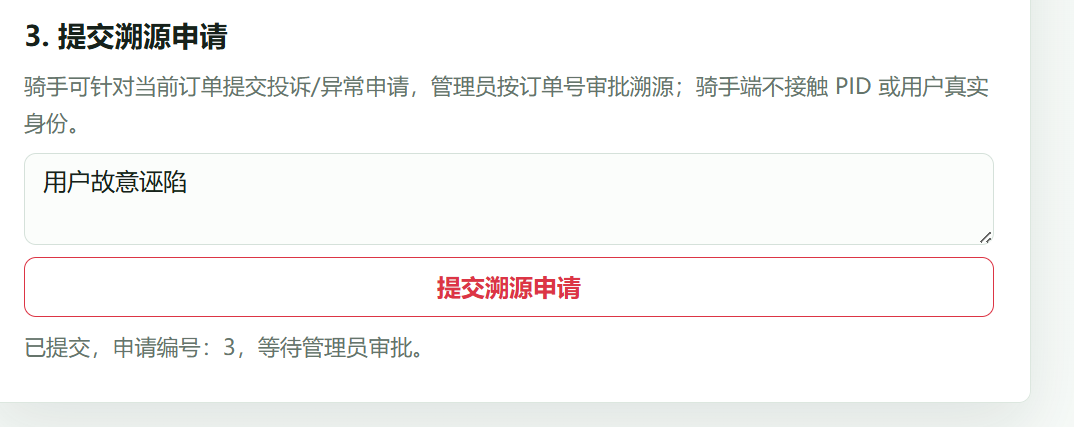
\includegraphics[width=0.85\textwidth]{content/chapter4/rider_trace_request.png}
    \caption{骑手端异常申请界面}
    \label{fig:rider-trace-request}
\end{figure}
